\documentclass[final]{beamer}
%% Possible paper sizes: a0, a0b, a1, a2, a3, a4.
%% Possible orientations: portrait, landscape
%% Font sizes can be changed using the scale option.
\usepackage[size=a0,orientation=portrait,scale=1.1]{beamerposter}

\usetheme{gemini}
\usecolortheme{smu}
\useinnertheme{rectangles}

% ====================
% Packages
% ====================

\usepackage[utf8]{inputenc}
\usepackage{graphicx}
\usepackage{booktabs}
\usepackage{tikz}
\usepackage{pgfplots}

% =====================
% Packages added by me
% =====================

\usepackage{chemformula} % para fórmulas químicas
\usepackage{mhchem}      % alternativa para ecuaciones químicas
\usepackage[backend=biber,style=numeric]{biblatex}
\usepackage{float}

% ====================
% Lengths
% ====================

% If you have N columns, choose \sepwidth and \colwidth such that
% (N+1)*\sepwidth + N*\colwidth = \paperwidth
\newlength{\sepwidth}
\newlength{\colwidth}
\setlength{\sepwidth}{0.03\paperwidth}
\setlength{\colwidth}{0.45\paperwidth}

\newcommand{\separatorcolumn}{\begin{column}{\sepwidth}\end{column}}

% ====================
% Logo (optional)
% ====================

% LaTeX logo taken from https://commons.wikimedia.org/wiki/File:LaTeX_logo.svg
% use this to include logos on the left and/or right side of the header:
\logoright{
\includegraphics[height=8cm]{logos/logo-right.png}}
\logoleft{
\includegraphics[height=8cm]{logos/logo-left.png}}

% ====================
% Footer (optional)
% ====================

\footercontent{
	ABC Conference 2025, Tokyo, Japan \hfill
	\insertdate \hfill
	\href{mailto:myemail@exampl.com}{\texttt{myemail@example.com}}
}
% (can be left out to remove footer)

% ====================
% My own customization
% - BibLaTeX
% - Boxes with tcolorbox
% - User-defined commands
% ====================
% ====================
% BibLaTeX
% ====================

%\usepackage[backend=biber,
%	bibstyle=authoryear,
%	citestyle=authoryear,
%	style=numeric,
%	maxcitenames=2,
%	maxbibnames=20, % limit the length of list of names (authors/editors/etc.)
%	sorting=none, % sort references by year (descending), name, title
%	dashed=false, % show authors instead of dash in publications having the same authors
%	giveninits=true % render authors' given name initials and not the full given names
%	oi=false, url=false
%]{biblatex}
%% Biblatex with Beamer bibliography icons
\setbeamertemplate{bibliography item}{%
	\ifboolexpr{ test {\ifentrytype{book}} or test {\ifentrytype{mvbook}}
		or test {\ifentrytype{collection}} or test {\ifentrytype{mvcollection}}
		or test {\ifentrytype{reference}} or test {\ifentrytype{mvreference}} }
	{\setbeamertemplate{bibliography item}[book]}
	{\ifentrytype{online}
		{\setbeamertemplate{bibliography item}[online]}
		{\setbeamertemplate{bibliography item}[article]}}%
	\usebeamertemplate{bibliography item}}
\defbibenvironment{bibliography}
{\list{}
	{\settowidth{\labelwidth}{\usebeamertemplate{bibliography item}}%
		\setlength{\leftmargin}{\labelwidth}%
		\setlength{\labelsep}{\biblabelsep}%
		\addtolength{\leftmargin}{\labelsep}%
		\setlength{\itemsep}{\bibitemsep}%
		\setlength{\parsep}{\bibparsep}}}
{\endlist}
{\item}
%% Redefine \refname
\renewcommand{\bibname}{References}
%% Redefine \parencite to use square brackets instead of braces
\DeclareCiteCommand{\parencite}
{\usebibmacro{prenote}}
{\usebibmacro{citeindex}%
	\printtext[bibhyperref]{[\usebibmacro{cite}]}}
{\multicitedelim}
{\usebibmacro{postnote}}
%% Highlight author names using Beamer data annotation
%% Usage: add a new line `author+an = {<author-order>=highlight}` to an entry
%% For example: author+an = {3=highlight} => highlight the 3rd author name
\AtBeginBibliography{
	\renewcommand*{\mkbibnamegiven}[1]{%
		\ifitemannotation{highlight}
		{\textbf{#1}}
		{#1}%
	}
	
	\renewcommand*{\mkbibnamefamily}[1]{%
		\ifitemannotation{highlight}
		{\textbf{#1}}
		{#1}%
	}
}

% ====================
% Boxes with tcolorbox
% ====================
\usepackage[most]{tcolorbox}

%%% Beamer colors in boxes

\newcommand{\beamercolorsinboxes}[1]{
	\setbeamercolor{itemize item}{fg=#1!75!black}
	\setbeamercolor{itemize/enumerate body}{fg=#1!65!white}
	\setbeamercolor{itemize/enumerate subbody}{fg=#1!65!white}
	\setbeamercolor{item projected}{fg=white, bg=#1!75!black}
}

%%% Highlight Oval Box
\newtcbox{\xmybox}[1][red]{on line,
	arc=7pt,colback=#1!10!white,colframe=#1!50!black,
	before upper={\rule[-3pt]{0pt}{10pt}},boxrule=1pt,
	boxsep=0pt,left=6pt,right=6pt,top=2pt,bottom=2pt}
%%% Box for stating problems
%%%%%%%%
%Usage: (similar for infobox)
%	\begin{defbox}{title}
	%		contents
	%	\end{defbox}
%%%%%%%%
\newtcolorbox{defbox}[1]{%
	enhanced,
	attach boxed title to top 	left={xshift=5mm,yshift=-5mm,yshifttext=-5mm},
	colback=cyan!5!white,
	colframe=cyan!75!black,
	coltitle=cyan!80!black,
%	left=0mm,right=0mm,top=2mm,bottom=0mm,
	title={#1},
	fonttitle=\bfseries\large, fontupper=\color{cyan!65!white},
	boxed title style={colback=cyan!5!white,colframe=cyan!75!black},
	before upper={
		\beamercolorsinboxes{cyan}
	}
}%
%%% Box for announcement
\newtcolorbox{infobox}[1]{%
	enhanced,
	attach boxed title to top 	left={xshift=5mm,yshift=-5mm,yshifttext=-5mm},
	colback=yellow,
	colframe=red!75!black,
	coltitle=red!75!black,
%	left=0mm,right=0mm,top=2mm,bottom=0mm,
	title={#1},
	fonttitle=\bfseries\large, fontupper=\color{red!65!white},
	boxed title style={colback=yellow,colframe=red!75!black},
	before upper={
		\beamercolorsinboxes{red}
	}
}%
%%% Box for example
\newtcolorbox{exabox}[1]{%
	enhanced,
	attach boxed title to top 	left={xshift=5mm,yshift=-5mm,yshifttext=-5mm},
	colframe=brown!75!black,colback=brown!5!white,coltitle=brown!50!brown!75!black,
%	left=0mm,right=0mm,top=2mm,bottom=0mm,
	title={#1},
	fonttitle=\bfseries\large, fontupper=\color{brown!65!white},
	boxed title style={colback=brown!5!white,coltitle=brown!50!brown!75!black},
	before upper={
		\beamercolorsinboxes{brown}
	}
}%
%%% Theorem Box
%%%%%%%%
%Usage: (similar for conjecture, lemma, etc.)
%	\begin{thm}{title}{nameref}
	%		contents
	%	\end{thm}
% Use \ref{thm:nameref} to refer to the theorem
%%%%%%%%
%%%% Use \newtcbtheorem[number within=section]{thm} to number within each section
\newtcbtheorem[]{thm}%
{Theorem}{attach boxed title to top 	left={xshift=5mm,yshift=-5mm,yshifttext=-5mm},
	enhanced jigsaw,
	%	top=2mm,bottom=0mm,left=0mm,right=0mm,
	fonttitle=\bfseries\large,fontupper=\itshape\color{blue!65!white},
	colframe=blue!75!black,colback=blue!5!white,coltitle=blue!50!blue!75!black,
	boxed title style={colback=blue!5!white,coltitle=blue!50!blue!75!black},
	before upper={
		\beamercolorsinboxes{blue}
	}
}{thm}%
%%% Proposition Box
\newtcbtheorem[use counter from=thm]{prop}%
{Proposition}{attach boxed title to top 	left={xshift=5mm,yshift=-5mm,yshifttext=-5mm},
	enhanced jigsaw,
	%	top=2mm,bottom=0mm,left=0mm,right=0mm,
	fonttitle=\bfseries\large,fontupper=\itshape,
	colframe=gray!75!black,colback=gray!5!white,coltitle=gray!50!gray!75!black,
	boxed title style={colback=gray!5!white,coltitle=gray!50!gray!75!black},
	before upper={
		\beamercolorsinboxes{gray}
	}
}{prop}%
%%% Conjecture Box
\newtcbtheorem[use counter from=thm]{conj}%
{Conjecture}{attach boxed title to top 	left={xshift=5mm,yshift=-5mm,yshifttext=-5mm},
	enhanced jigsaw,
	%	top=2mm,bottom=0mm,left=0mm,right=0mm,
	fonttitle=\bfseries\large,fontupper=\slshape,
	colframe=orange!75!black,colback=orange!5!white,coltitle=orange!50!orange!75!black,
	boxed title style={colback=orange!5!white,coltitle=orange!50!orange!75!black},
	before upper={
		\beamercolorsinboxes{orange}
	}
}{conj}%
%%% Lemma Box
\newtcbtheorem[use counter from=thm]{lem}%
{Lemma}{attach boxed title to top 	left={xshift=5mm,yshift=-5mm,yshifttext=-5mm},
	enhanced jigsaw,
	%	top=2mm,bottom=0mm,left=0mm,right=0mm,
	fonttitle=\bfseries\large,fontupper=\itshape,
	colframe=green!75!black,colback=green!5!white,coltitle=green!50!green!75!black,
	boxed title style={colback=green!5!white,coltitle=green!50!green!75!black},
	before upper={
		\beamercolorsinboxes{green}
	}
}{lem}%
%%% Claim Box
\newtcbtheorem[use counter from=thm]{clm}%
{Claim}{attach boxed title to top 	left={xshift=5mm,yshift=-5mm,yshifttext=-5mm},
	enhanced jigsaw,
	%	top=2mm,bottom=0mm,left=0mm,right=0mm,
	fonttitle=\bfseries\large,fontupper=\itshape,
	colframe=pink!75!black,colback=pink!5!white,coltitle=pink!50!pink!75!black,
	boxed title style={colback=pink!5!white,coltitle=pink!50!pink!75!black},
	before upper={
		\beamercolorsinboxes{pink}
	}
}{clm}%

%% Reference Sources
\addbibresource{referencias.bib}
\renewcommand{\pgfuseimage}[1]{\includegraphics[scale=2.0]{#1}}

\title{Estudio de la solvatación del ion \ce{Cu^{2+}} en medios polares mediante dinámica molecular con DFT/M06-2X}

\author{Jorge Angel Rosas Martínez \inst{1} \and César Iván León Pimentel \inst{2}}
\institute[shortinst]{\inst{1} Facultad de Química, UNAM }

\date{Agosto 2025}

\begin{document}
	
\begin{frame}[t]
	
	\begin{columns}[t]
		\separatorcolumn

		\begin{column}{\colwidth}
			\begin{block}{Introducción}
				El ion \ce{Cu^{2+}} desempeña un papel fundamental en reacciones de oxidación-reducción, transporte electrónico y formación de complejos metaloproteicos, procesos estrechamente ligados a funciones fisiológicas clave y a enfermedades neurodegenerativas como el Alzheimer y el Parkinson \cite{Me-2022-01}. Tiene aplicaciones en el diseño de fármacos, catálisis homogénea, sensorización iónica, y en el análisis molecular de sistemas biológicos \cite{Me-2023-01}. En este estudio, se analizaron los sistemas \ce{[Cu(H2O)_{40}]^{2+}} y \ce{[Cu(CH3OH)_{40}]^{2+}}, con el objetivo de hacer un análisis estructural y energético mediante simulaciones de dinámica molecular a 300 K durante 22.5 ps.

			\end{block}

			
		\end{column}

		\separatorcolumn

		\begin{column}{\colwidth}
			\begin{block}{Metodología}
				Las simulaciones de dinámica molecular de Born-Oppenheimer se llevaron a cabo en el programa ORCA v6.1 \cite{orca6.1}, utilizando condiciones de ensamble NVT y control de temperatura mediante un termostato de Nosé-Hoover en cadena. Las velocidades iniciales se generaron conforme a la distribución de Maxwell-Boltzmann a 300 K.

				ORCA integra el movimiento atómico empleando el algoritmo de Verlet de velocidad, y en cada paso temporal resuelve la ecuación de Schrödinger independiente del tiempo mediante el método de campo autoconsistente y teoría de los fucionales de la densidad (SCF-DFT por sus siglas en inglés), utilizando el funcional M06-2X y el nivel de teoría 6-31G$^\ast$. Este procedimiento permite obtener las fuerzas necesarias para la evolución del sistema conforme a las ecuaciones de movimiento de Newton.
			\end{block}			
		\end{column}
		
		\separatorcolumn
	
	\end{columns}

	\begin{columns}[t]
	
		\begin{column}{2\colwidth+\sepwidth}
			\begin{alertblock}{Introducción}

				Las siguientes figuras son representativas:

				\begin{figure}[H]
					\centering
					\begin{minipage}[b]{0.25\textwidth}
						\centering
						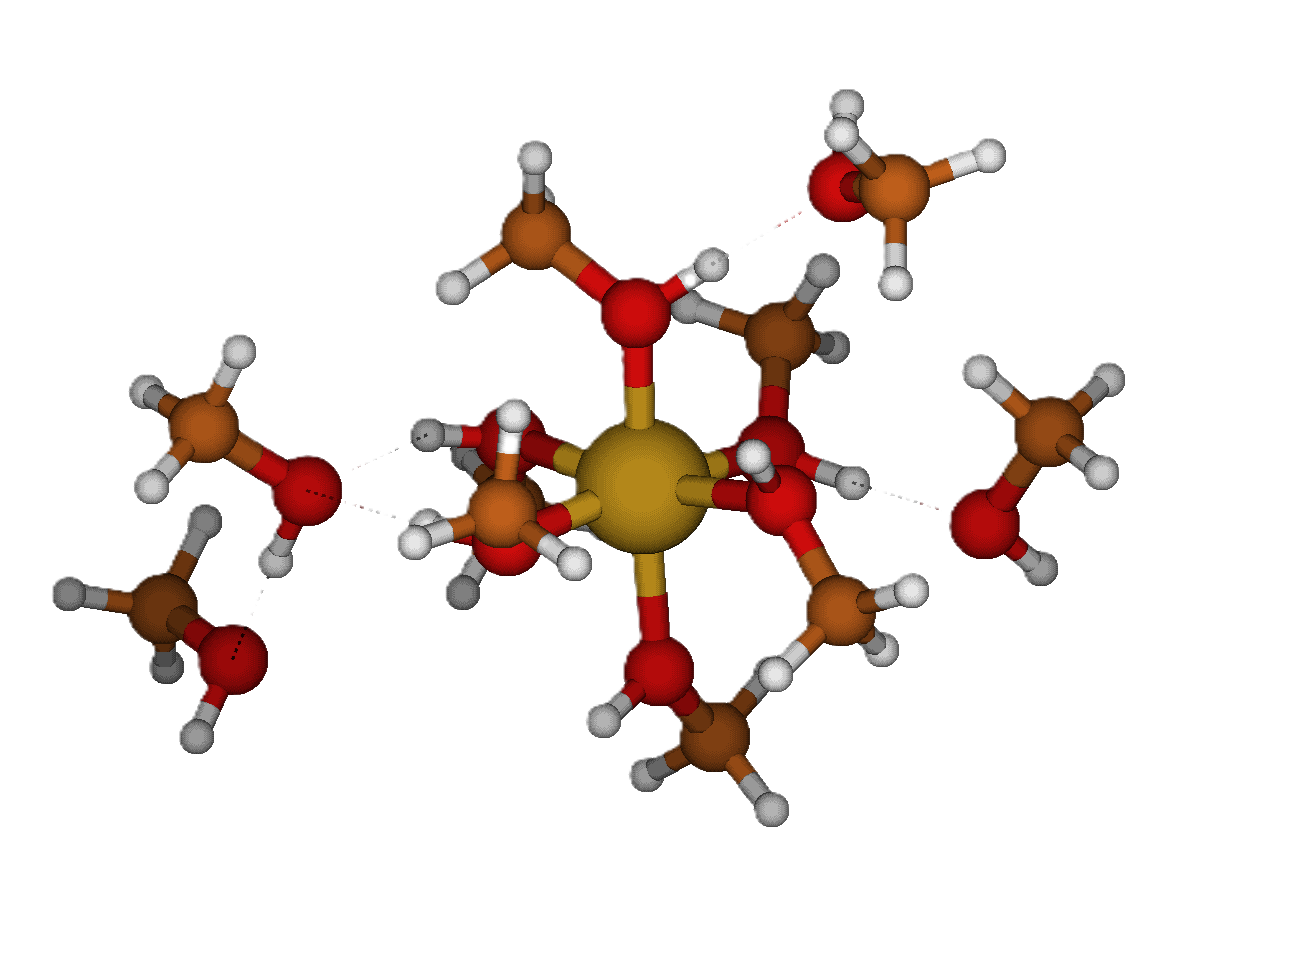
\includegraphics[width=\textwidth]{logos/Cu-10CH4O.png}
					\end{minipage}%
					\hfill
					\begin{minipage}[b]{0.25\textwidth}
						\centering
						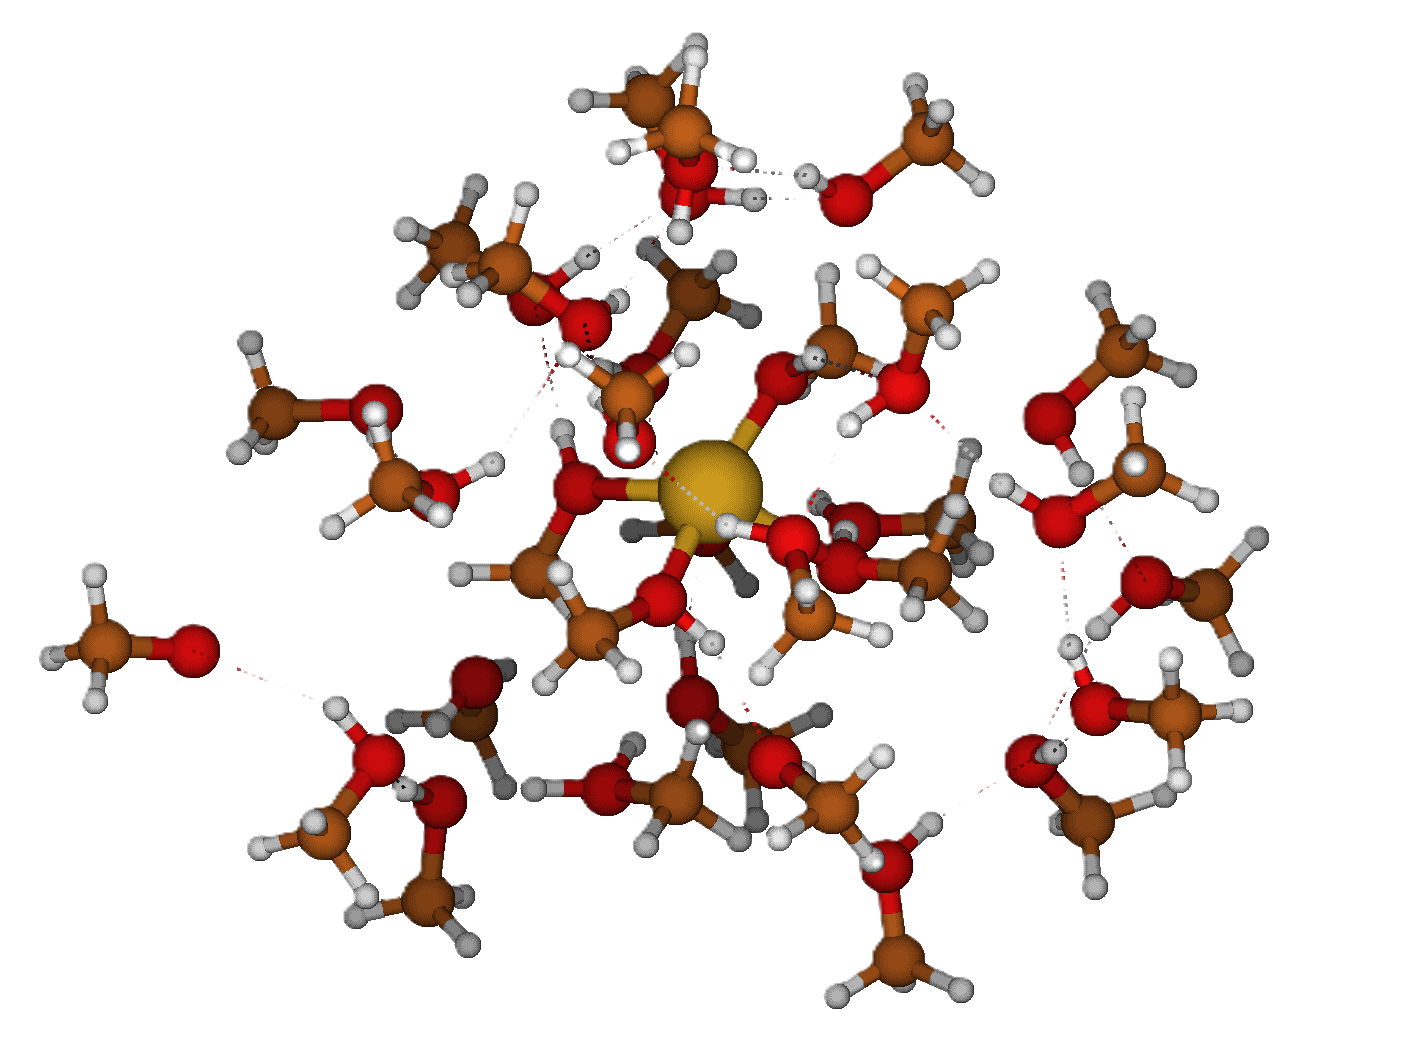
\includegraphics[width=\textwidth]{logos/Cu-30CH4O.png}
					\end{minipage}
					\hfill
					\begin{minipage}[b]{0.25\textwidth}
						\centering
						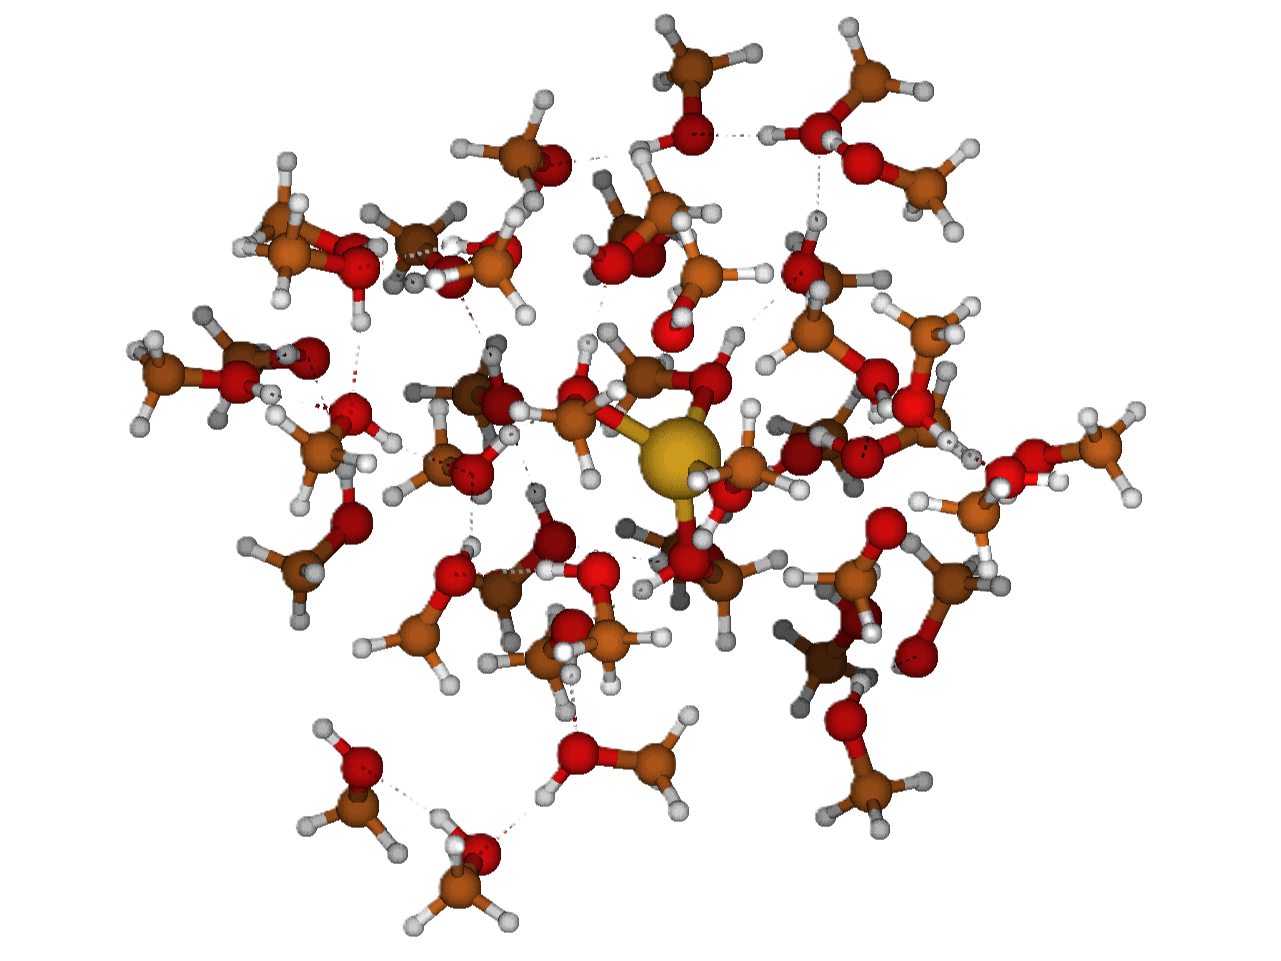
\includegraphics[width=\textwidth]{logos/Cu-40CH4O.png}
					\end{minipage}

					\caption{Energías de enlace por molécula de solvente calculada para las estructuras de solvatación óptimas de \ce{[Cu(H2O)_{n}]^{2+}} (izquierda) y \ce{[Cu(CH3OH)_{n}]^{2+}} (derecha), con $n = 1,\ 2,\ \ldots,\ 10,\ 30,\ 40$, mediante cálculos de optimización con los niveles de teoría 6-31G$^\ast$, 6-31+G$^\ast$ y 6-31++G$^{\ast\ast}$. Se concluye que la base 6-31G$^\ast$ ofrece un buen equilibrio entre precisión y costo computacional. Gráficas pendientes}
					\label{fig:bases}
				\end{figure}	

				\begin{figure}[H]
					\centering
					\begin{minipage}[b]{0.25\textwidth}
						\centering
						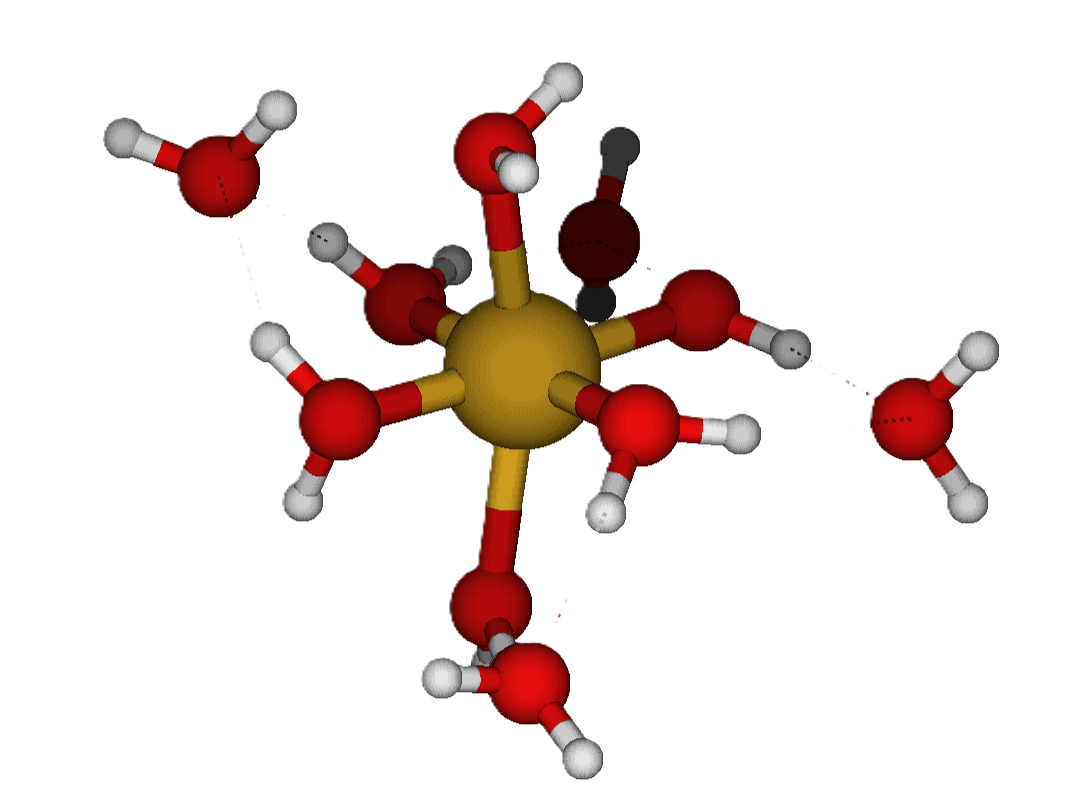
\includegraphics[width=\textwidth]{logos/Cu-10H2O.png}
					\end{minipage}%
					\hfill
					\begin{minipage}[b]{0.25\textwidth}
						\centering
						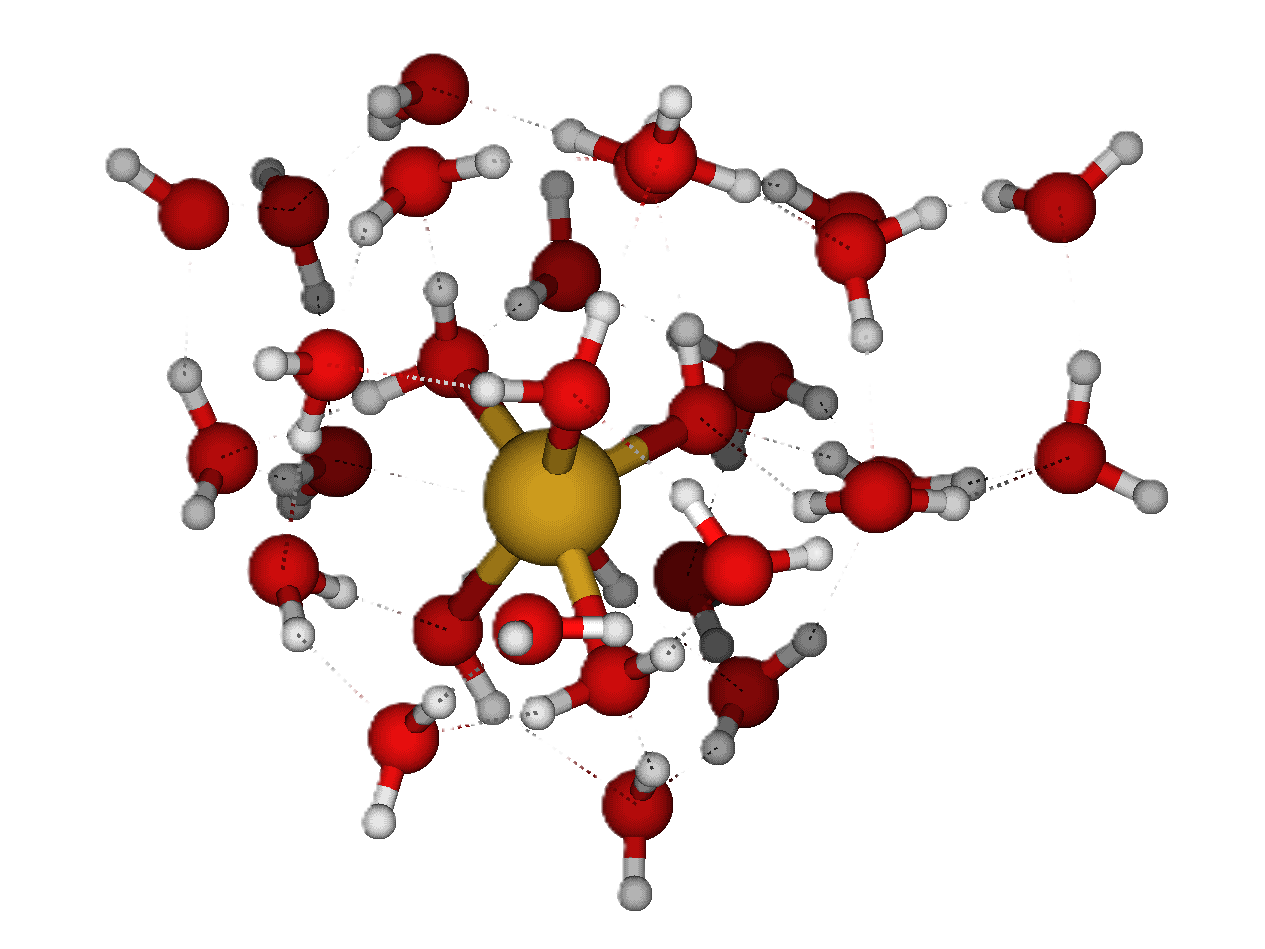
\includegraphics[width=\textwidth]{logos/Cu-30H2O.png}
					\end{minipage}
					\hfill
					\begin{minipage}[b]{0.25\textwidth}
						\centering
						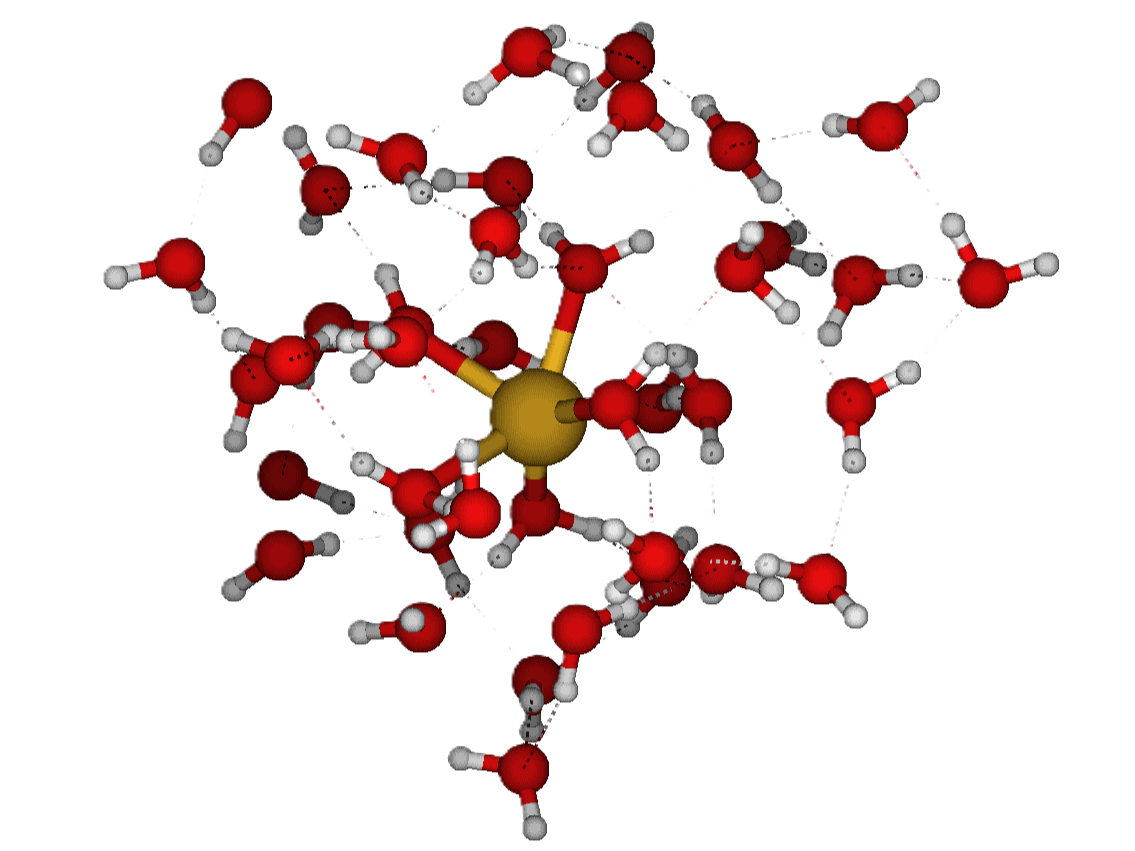
\includegraphics[width=\textwidth]{logos/Cu-40H2O.png}
					\end{minipage}

					\caption{Energías de enlace por molécula de solvente calculada para las estructuras de solvatación óptimas de \ce{[Cu(H2O)_{n}]^{2+}} (izquierda) y \ce{[Cu(CH3OH)_{n}]^{2+}} (derecha), con $n = 1,\ 2,\ \ldots,\ 10,\ 30,\ 40$, mediante cálculos de optimización con los niveles de teoría 6-31G$^\ast$, 6-31+G$^\ast$ y 6-31++G$^{\ast\ast}$. Se concluye que la base 6-31G$^\ast$ ofrece un buen equilibrio entre precisión y costo computacional. Gráficas pendientes}
					\label{fig:bases}
				\end{figure}


			\end{alertblock}
		\end{column}

	\end{columns}

	\begin{columns}[t]

		\separatorcolumn
		
		\begin{column}{\colwidth}
			
			\begin{block}{An example block containing some math}{}

				%%%
				\begin{figure}[H]
					\centering
					\begin{minipage}[b]{0.48\textwidth}
						\centering
						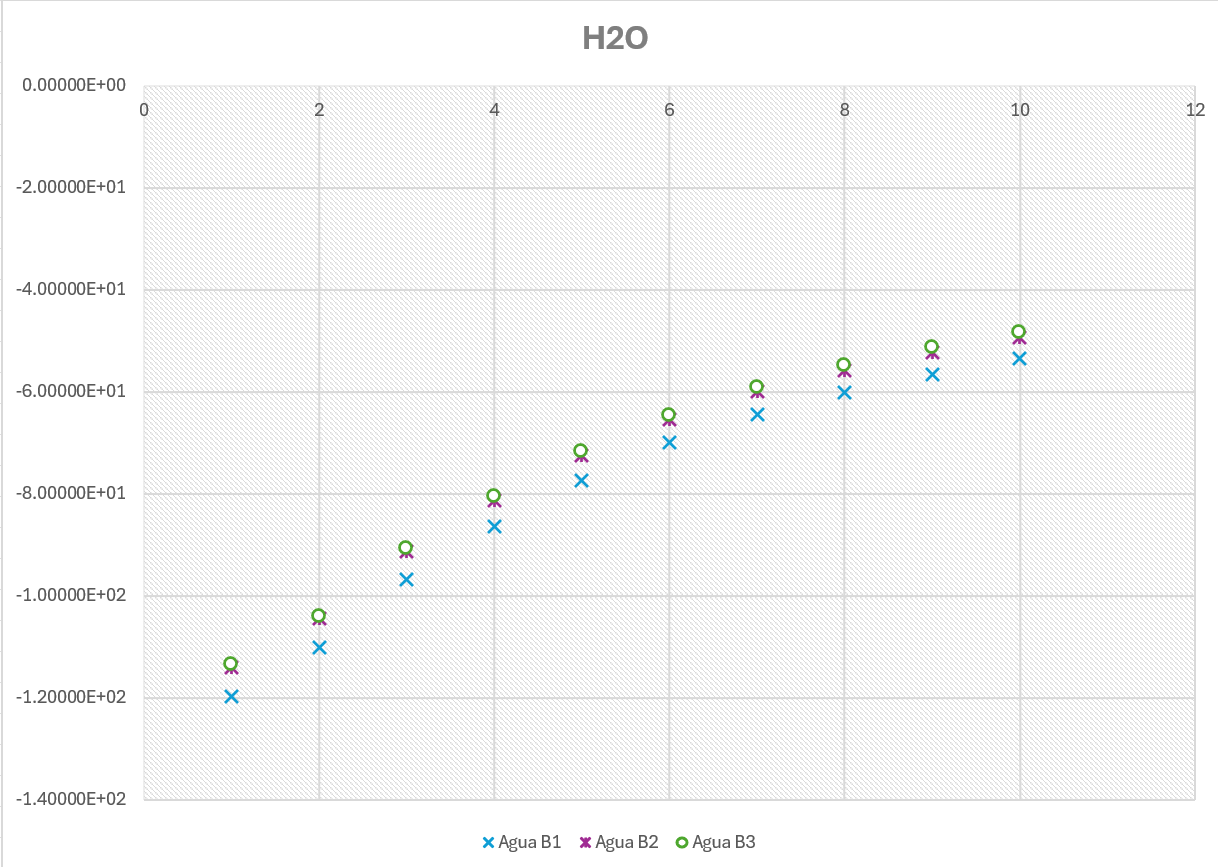
\includegraphics[width=\textwidth]{logos/bases_agua.png}
					\end{minipage}%
					\hfill
					\begin{minipage}[b]{0.48\textwidth}
						\centering
						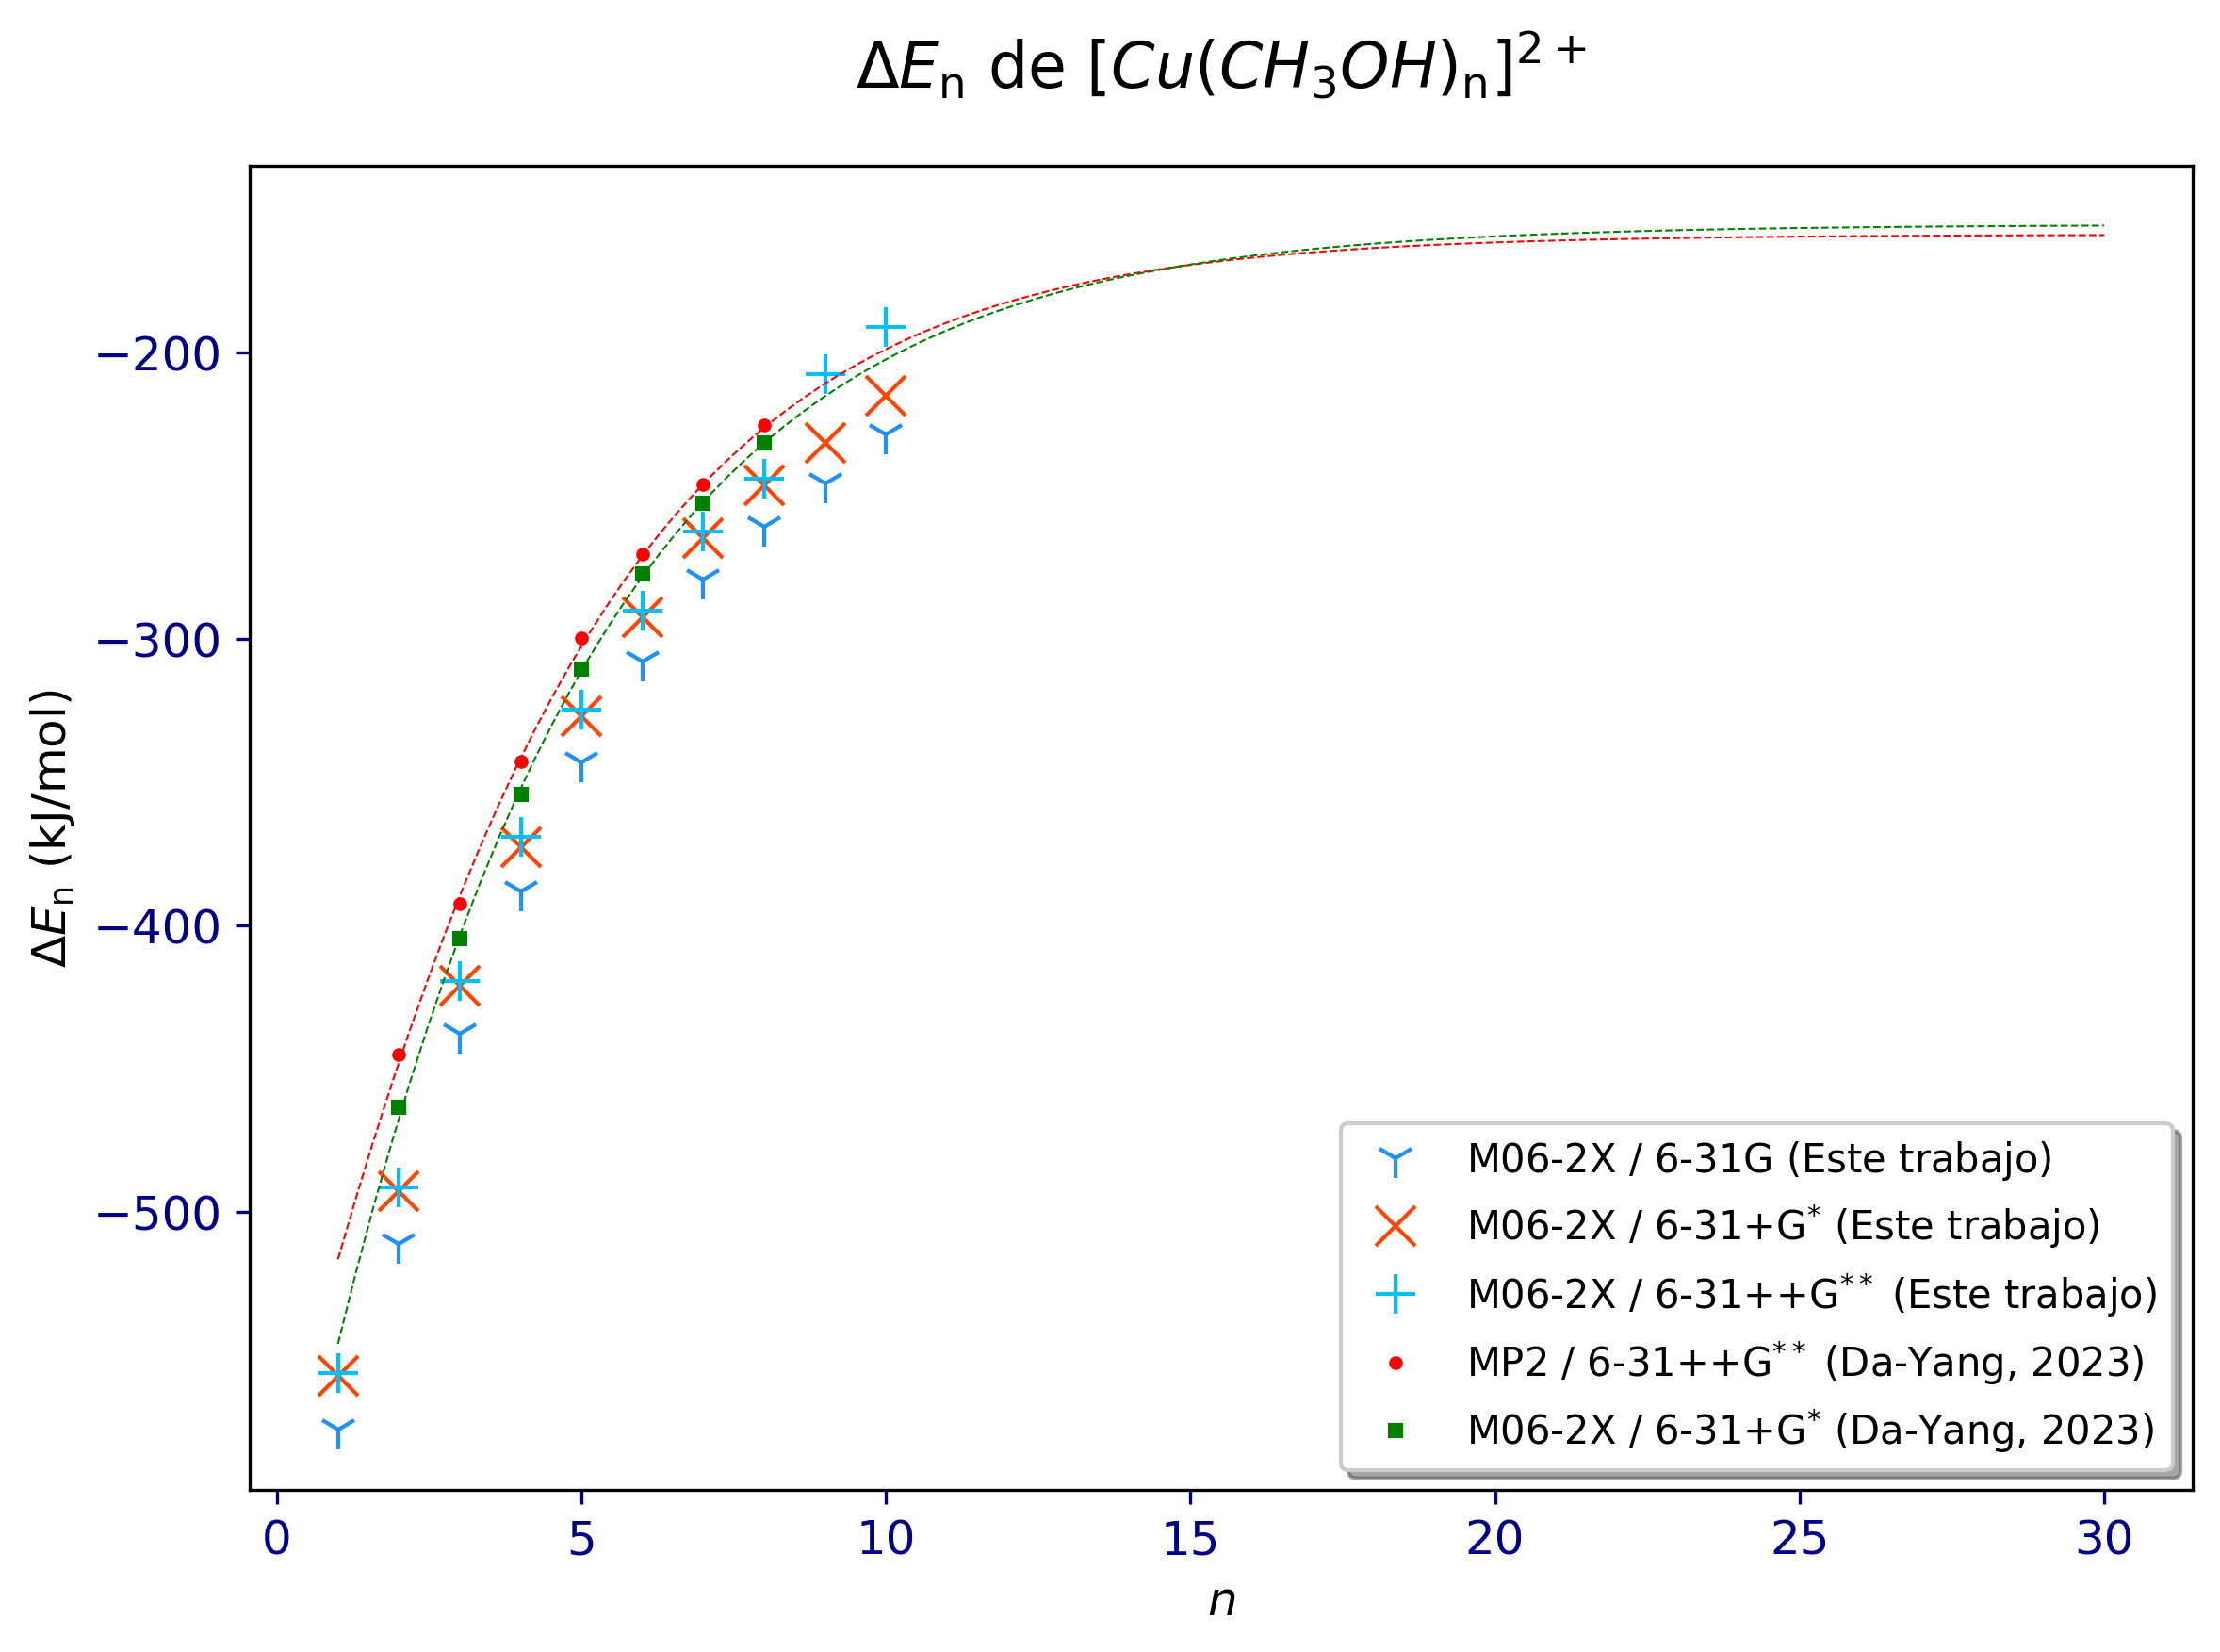
\includegraphics[width=\textwidth]{logos/bases_metanol.png}
					\end{minipage}

					\caption{Energías de enlace por molécula de solvente calculada para las estructuras de solvatación óptimas de \ce{[Cu(H2O)_{n}]^{2+}} (izquierda) y \ce{[Cu(CH3OH)_{n}]^{2+}} (derecha), con $n = 1,\ 2,\ \ldots,\ 10,\ 30,\ 40$, mediante cálculos de optimización con los niveles de teoría 6-31G$^\ast$, 6-31+G$^\ast$ y 6-31++G$^{\ast\ast}$. Se concluye que la base 6-31G$^\ast$ ofrece un buen equilibrio entre precisión y costo computacional. Gráficas pendientes}
					\label{fig:bases}
				\end{figure}
				
			\end{block}
			
			\begin{block}{An example block containing some math}{}
				
				\begin{figure}[H]
					\centering
					% Primera imagen
					\begin{minipage}[c]{0.49\textwidth} % Adjust width as needed, ensure total < 1.0\textwidth
						\centering
						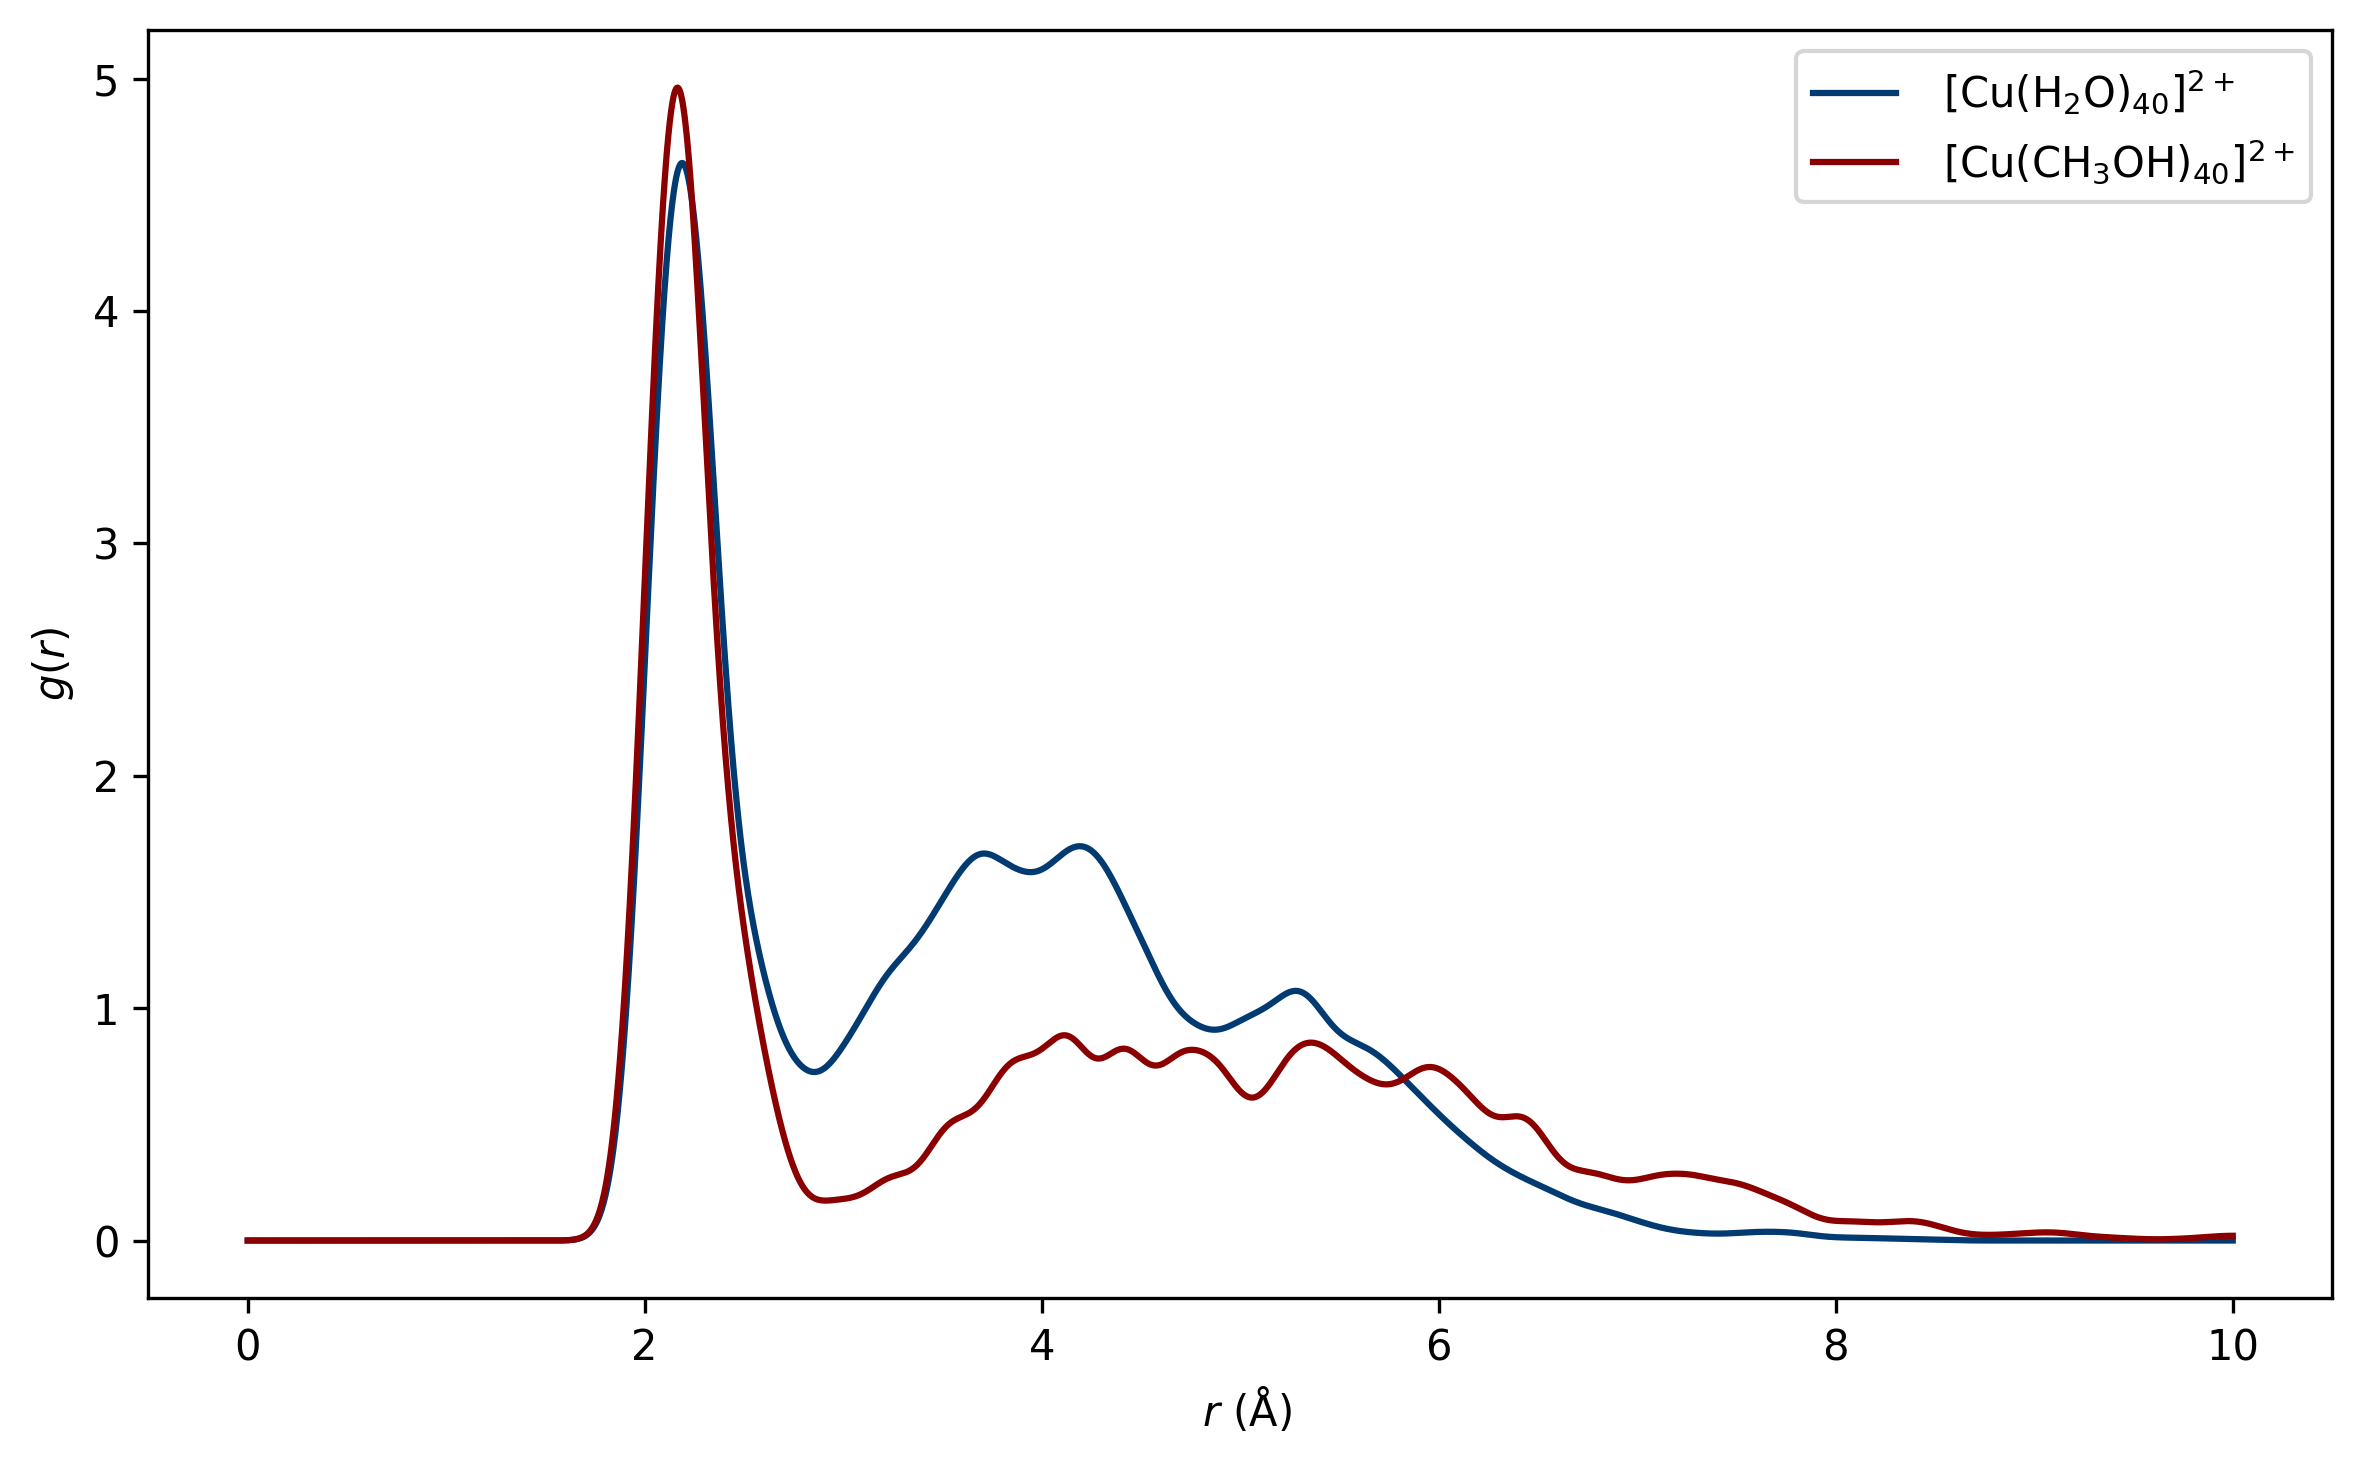
\includegraphics[width=\textwidth]{logos/RDF-OUTPUT-HISTOGRAMA.png}
						\caption{Función de distribución radial para el ion \ce{Cu^{2+}} en metanol (\ce{CH_{4}O}) y agua (\ce{H_{2}O}).}
						\label{fig:rdfcu40ch4o}
					\end{minipage}% <--- Important: No space here!
					\hfill % Adds flexible space between minipages, or remove if you want them tight
					% Segunda imagen
					\begin{minipage}[c]{0.49\textwidth} % Adjust width as needed
						\centering
						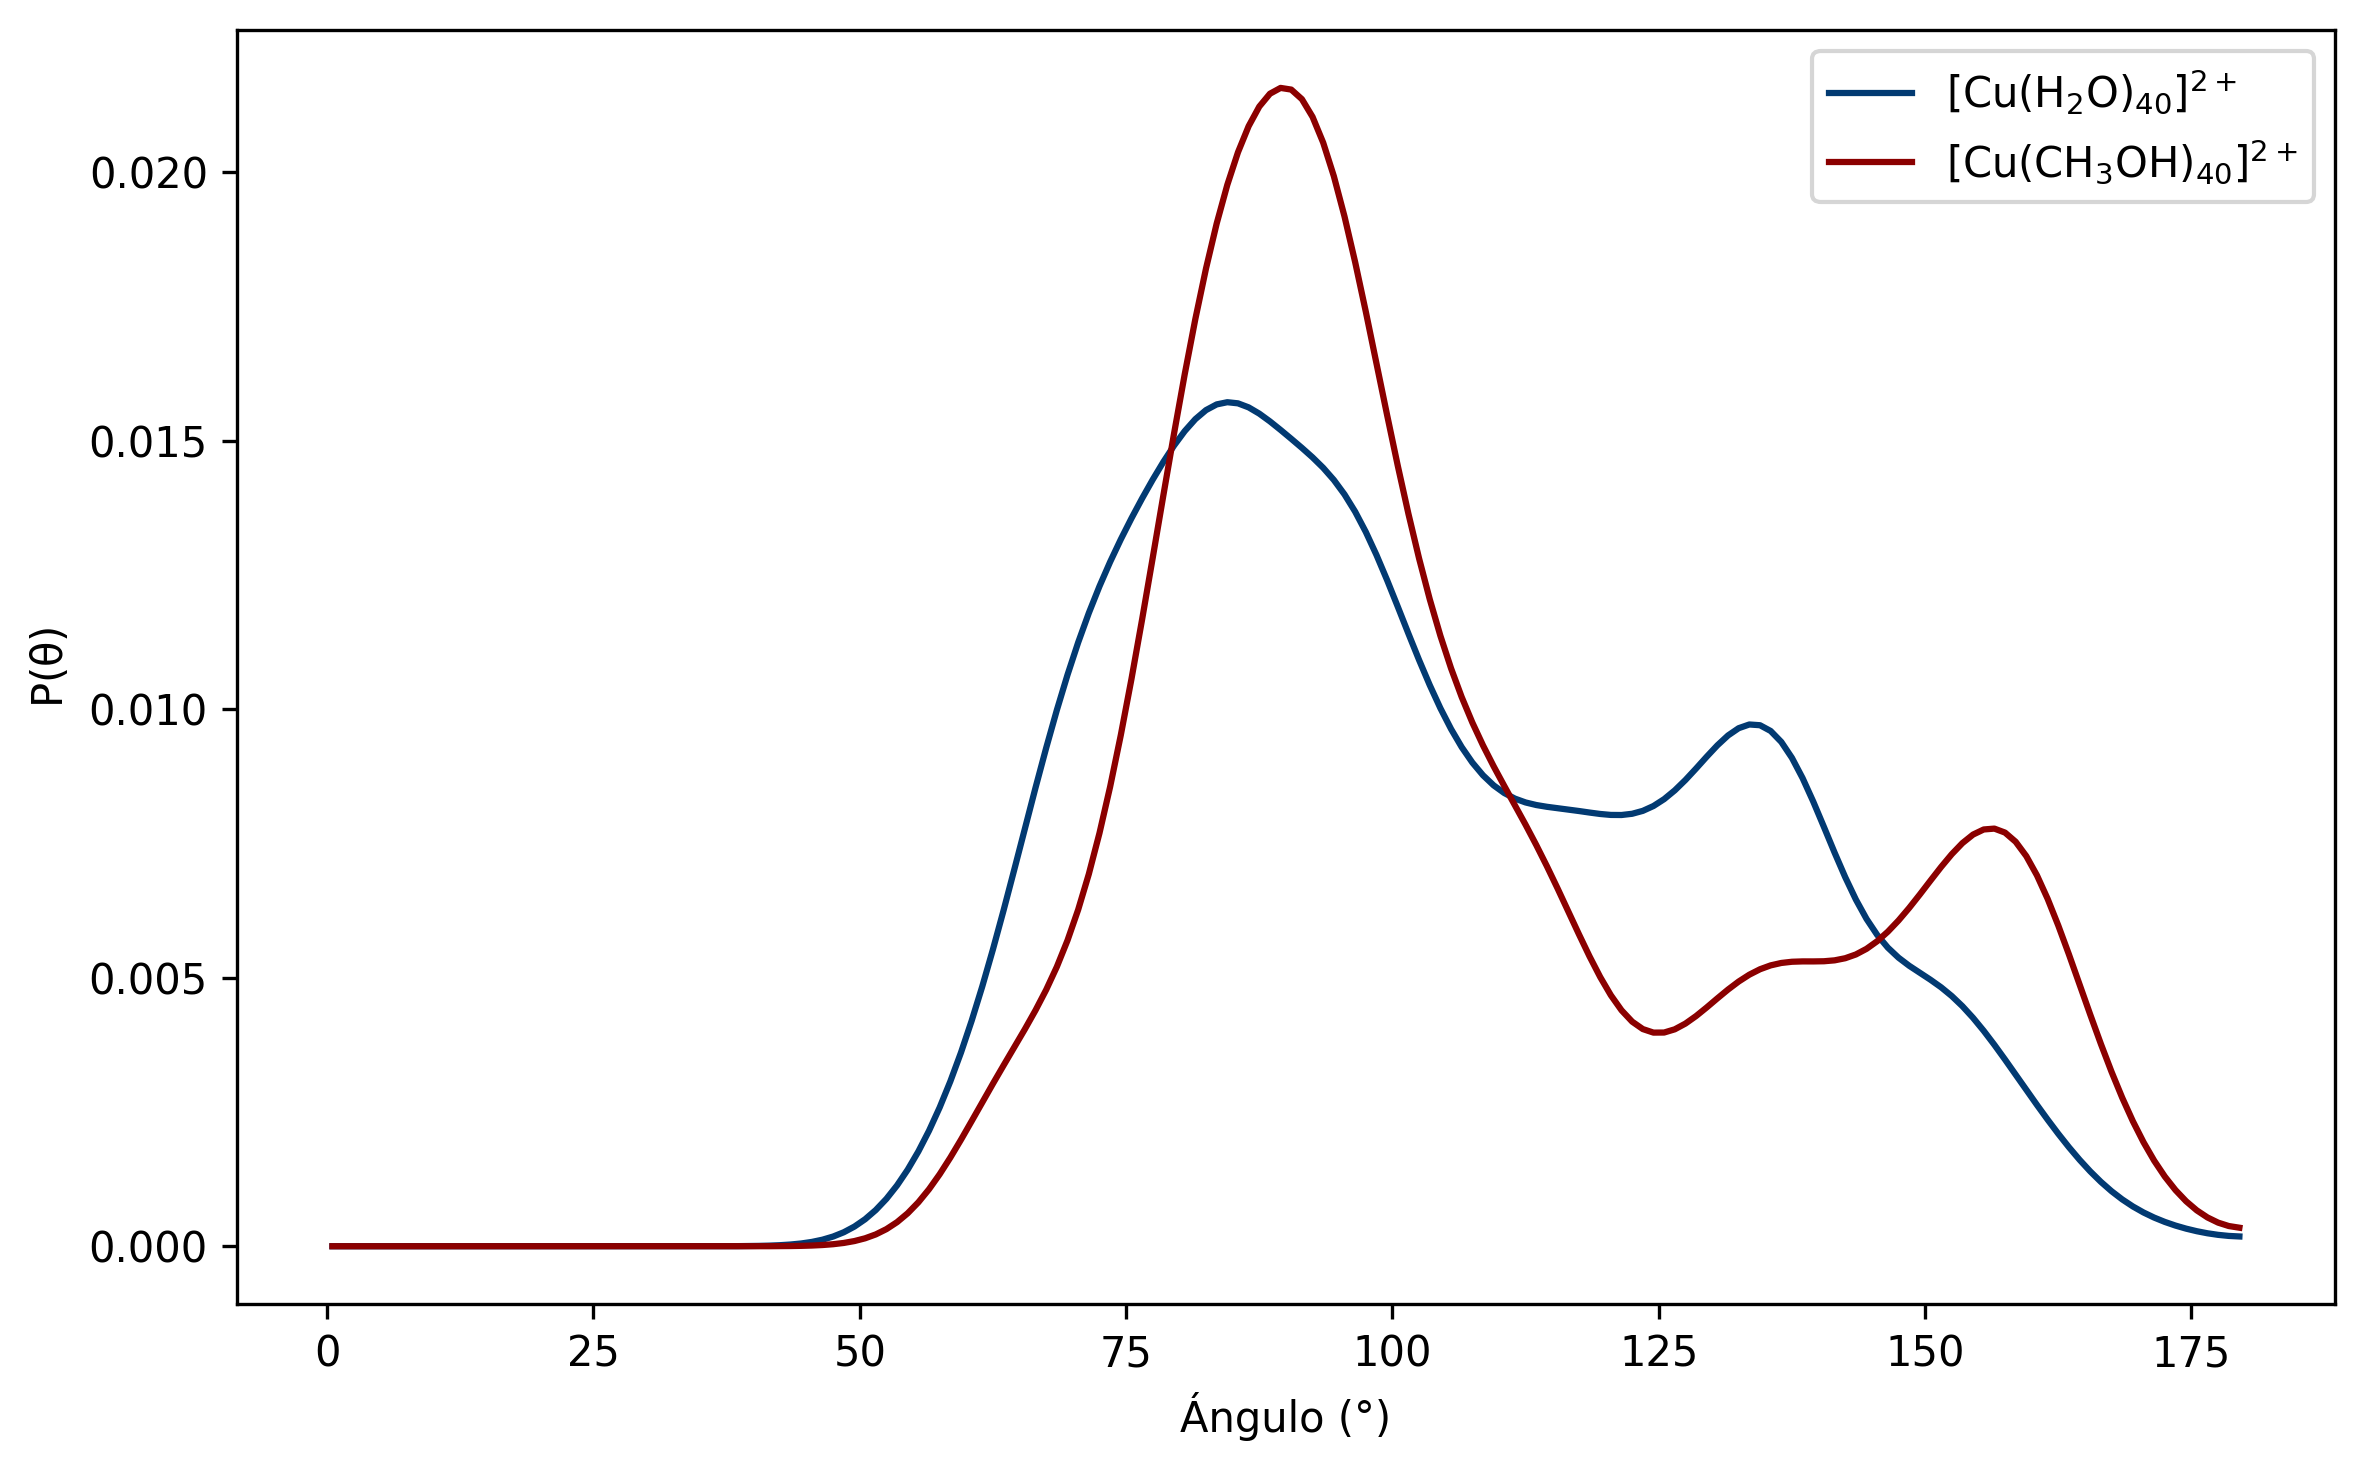
\includegraphics[width=\textwidth]{logos/ADF-OUTPUT-HISTOGRAMA.png}
						\caption{Función de distribución angular con $r = 2.9$ para el ion \ce{Cu^{2+}} en metanol (\ce{CH_{4}O}) y agua (\ce{H_{2}O}).}
						\label{fig:adfcu40ch4o}
					\end{minipage}
				\end{figure}

			\end{block}		

		\end{column}
	
		\separatorcolumn
		
		\begin{column}{\colwidth}

			\begin{exampleblock}{Resultados y discusión}
				Los resultados obtenidos muestran que la energía de enlace por molécula de solvente para \ce{[Cu(H2O)_{n}]^{2+}} y \ce{[Cu(CH3OH)_{n}]^{2+}} disminuye conforme aumenta el número de moléculas de solvente, lo que indica una mayor estabilidad del ion en medios polares. La función de distribución radial (RDF) y la función de distribución angular (ADF) revelan la estructura local del ion \ce{Cu^{2+}} en ambos solventes, mostrando una preferencia por ciertas distancias y ángulos entre las moléculas de agua y metanol.

				Los resultados sugieren que el ion \ce{Cu^{2+}} forma complejos más estables en metanol que en agua, lo cual es consistente con estudios previos sobre la solvatación de iones metálicos en medios polares.

				
			\end{exampleblock}					

			
			\begin{block}{References}
				\printbibliography[heading=none]
			\end{block}
		\end{column}
		
		\separatorcolumn
	\end{columns}
\end{frame}
\end{document}